\chapter{Выполнение работы}
\label{ch:chapter_radio}

\section{Исходные данные и параметры моделирования}

В таблице~\ref{tab:params} приведены исходные параметры моделирования
для обеих частей работы.

\begin{table}[h]
    \caption{Параметры моделирования}
    \label{tab:params}
    \centering
    \begin{tabular}{lll}
        \toprule
        Параметр & Обозначение & Значение \\
        \midrule
        Несущая частота              & $f_c$        & 2 ГГц \\
        Скорость света               & $c$          & $3\cdot10^8$ м/с \\
        Длина волны                  & $\lambda$    & $c/f_c = 0{,}15$ м \\
        Число отсчётов на $\lambda$  & $F$          & 16 \\
        Шаг по расстоянию            & $\Delta x$   & $\lambda/F$ \\
        Скорость абонента            & $V$          & 10 м/с \\
        Число точек траектории (ч.~1) & $N$         & 100 \\
        Число точек траектории (ч.~2) & $N$         & 1000 \\
        Размер ДПФ (ч.~1)            & $N_{\text{FFT}}$ & 128 \\
        Расстояние BS--MS (ч.~1)     & $D$          & 1000 м \\
        Координаты BS (ч.~2)         & $(x_{BS},y_{BS})$ & (1000; 1000) м \\
        \bottomrule
    \end{tabular}
\end{table}

Комплексная огибающая сигнала для одного луча вычисляется как
\begin{equation}
    r(n) = \exp\!\bigl(-j\,k\,d(n)\bigr), \qquad k = \frac{2\pi}{\lambda},
    \label{eq:envelope}
\end{equation}
где $d(n)$ — пройденное сигналом расстояние на $n$-м отсчёте траектории.

\section{Часть 1. Приём сигнала при прямом луче}

\subsection{Модель траектории и расстояний}

Абонент начинает движение в точке $x(0)=0$ и перемещается вдоль оси $X$
с шагом $\Delta x = \lambda/F$. Координаты отсчётных точек:
\begin{equation}
    x(n) = n\,\Delta x,\quad n = 0,1,\dots,N-1.
\end{equation}
Соответствующие моменты времени и интервал дискретизации:
\begin{equation}
    t(n) = \frac{n\,\Delta x}{V}, \qquad t_s = \frac{\Delta x}{V},
    \qquad f_s = \frac{1}{t_s}.
\end{equation}
Расстояние от BS до MS на $n$-м отсчёте при движении навстречу BS:
\begin{equation}
    d(n) = D - n\,\Delta x.
\end{equation}

Для общности координаты BS задаются как
$BS_x = D\cos\alpha$, $BS_y = D\sin\alpha$, а расстояние вычисляется по
теореме Пифагора:
\begin{equation}
    d_{BS\text{-}MS}(n) = \sqrt{(BS_x - MS_x(n))^2 + (BS_y - MS_y(n))^2}.
\end{equation}
В данной работе принято $\alpha = 0$ (BS на оси $X$), поэтому
$d_{BS\text{-}MS}(n) = D - n\Delta x$.

\subsection{Комплексная огибающая, амплитуда и фаза}

По формуле~\eqref{eq:envelope} вычислена комплексная огибающая $r(n)$.
На рисунке~\ref{fig:part1} приведены графики амплитуды, фазы, вещественной
части сигнала и доплеровского спектра.

\begin{figure}[h]
    \centering
    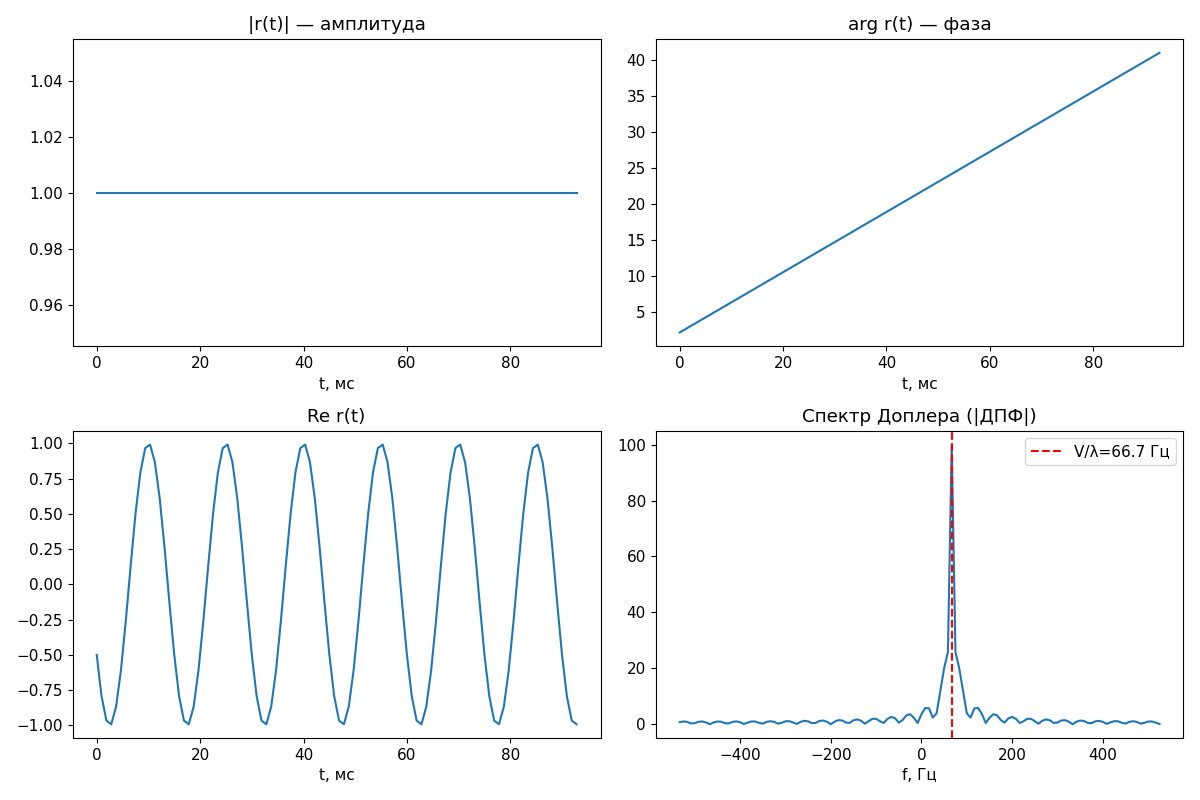
\includegraphics[width=\textwidth]{radio_part1.png}
    \caption{Часть 1: амплитуда, фаза, вещественная часть и спектр Доплера
             для прямого луча}
    \label{fig:part1}
\end{figure}

\textbf{Амплитуда.} Поскольку луч единственный и потерь не моделируется,
$|r(n)| = 1$ для всех $n$ — замираний нет.

\textbf{Фаза.} Фаза линейно убывает со временем:
\begin{equation}
    \arg r(n) = -k\,d(n) = -kD + k\,n\,\Delta x,
\end{equation}
что соответствует постоянному доплеровскому сдвигу.

\textbf{Доплеровский сдвиг.} Ось частот при ДПФ размечена как
\begin{equation}
    f_m = \left(-\frac{N_{\text{FFT}}}{2} + m\right)\frac{f_s}{N_{\text{FFT}}},
    \quad m = 0,1,\dots,N_{\text{FFT}}-1.
\end{equation}
Пик спектра соответствует теоретическому значению
\begin{equation}
    f_D = \frac{V}{\lambda} = \frac{10}{0{,}15} \approx 66{,}7~\text{Гц}.
\end{equation}
Для параметров работы $f_s = V/\Delta x = V F/\lambda \approx 1066{,}7$~Гц,
разрешение по частоте $\Delta f = f_s/N_{\text{FFT}} \approx 8{,}33$~Гц.
Пик ДПФ попадает в интервал, ближайший к $f_D$, что подтверждает
корректность модели.

\textbf{Вывод по части 1.} При наличии только прямого луча принимаемый
сигнал имеет постоянную амплитуду и линейно меняющуюся фазу; доплеровский
спектр представляет собой одиночную спектральную линию на частоте
$f_D = V/\lambda$. Замираний нет.

\section{Часть 2. Приём сигнала при большом числе источников переотражений}

\subsection{Сценарий моделирования}

Начальное положение абонента: $MS(0,0)$. Базовая станция:
$BS(1000;1000)$~м. Рассеиватели (Scatterers, SC) расположены вокруг
приёмника случайным образом в кольце радиусом от 50 до 300~м:
\begin{equation}
    x_{SC_i} = r_i\cos\varphi_i,\quad y_{SC_i} = r_i\sin\varphi_i,
    \quad r_i \sim U(50,300),\ \varphi_i \sim U(0,2\pi).
\end{equation}
Число рассеивателей $N_{SC} = 200$. Исходный сценарий показан на
рисунке~\ref{fig:scenario}.

\begin{figure}[h]
    \centering
    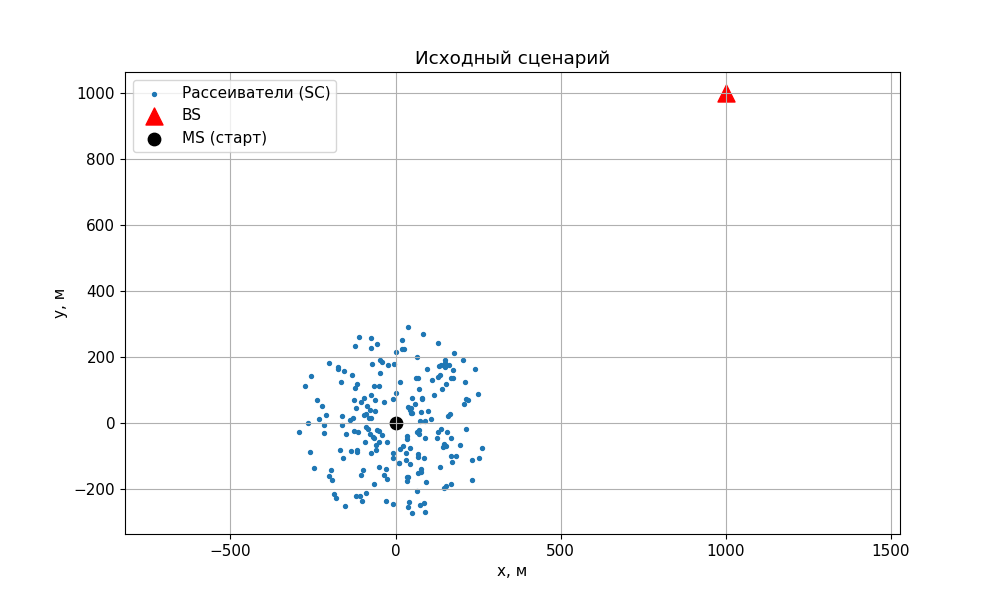
\includegraphics[width=0.8\textwidth]{radio_scenario.png}
    \caption{Исходный сценарий: BS, MS и рассеиватели}
    \label{fig:scenario}
\end{figure}

\subsection{Траектория перемещения абонента}

Абонент перемещается по линейному треку из $N = 1000$ точек со скоростью
$V = 10$~м/с. Длина трека принята $L = 300$~м, шаг по расстоянию
$\Delta x = L/(N-1)$. Трек и рассеиватели показаны на
рисунке~\ref{fig:track}.

\begin{figure}[h]
    \centering
    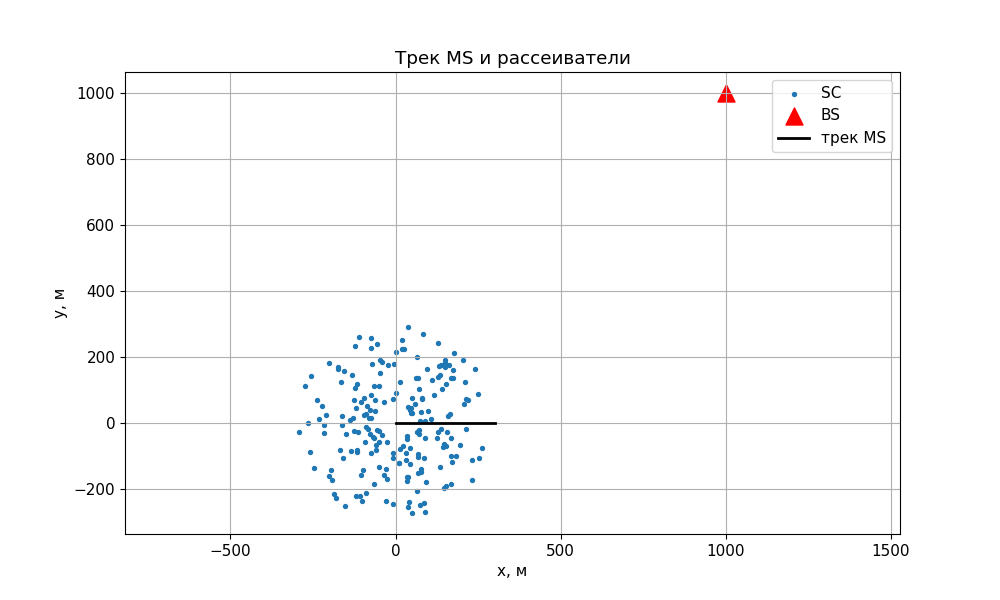
\includegraphics[width=0.8\textwidth]{radio_track.png}
    \caption{Трек перемещения абонента на карте с рассеивателями}
    \label{fig:track}
\end{figure}

\subsection{Расстояния BS--SC--MS}

Расстояния вычисляются для каждого $i$-го пути рассеивания в каждой $n$-й
точке траектории:
\begin{align}
    d_{BS\text{-}SC_i} &= \sqrt{(x_{BS} - x_{SC_i})^2 + (y_{BS} - y_{SC_i})^2},\\
    d_{SC_i\text{-}MS}(n) &= \sqrt{(x_{SC_i} - x_{MS}(n))^2 + (y_{SC_i} - y_{MS}(n))^2}.
\end{align}
Суммарное расстояние по $i$-му пути:
\begin{equation}
    d_i(n) = d_{BS\text{-}SC_i} + d_{SC_i\text{-}MS}(n).
\end{equation}

\subsection{Принимаемый сигнал}

Комплексная амплитуда $i$-го пути с учётом случайной начальной фазы
$\varphi_{0i}$:
\begin{equation}
    r_i(n) = \exp\!\bigl(j\varphi_{0i} - j\,k\,d_i(n)\bigr).
\end{equation}
Суммарный принимаемый сигнал:
\begin{equation}
    r(n) = \frac{1}{\sqrt{N_{SC}}}\sum_{i=1}^{N_{SC}} r_i(n).
\end{equation}
Нормировка $1/\sqrt{N_{SC}}$ сохраняет среднюю мощность сигнала
$\mathbb{E}|r|^2 \approx 1$.

\subsection{Характеристики принимаемого сигнала}

На рисунке~\ref{fig:part2} приведены модуль, фаза, вещественная часть
принятого сигнала и доплеровский спектр.

\begin{figure}[h]
    \centering
    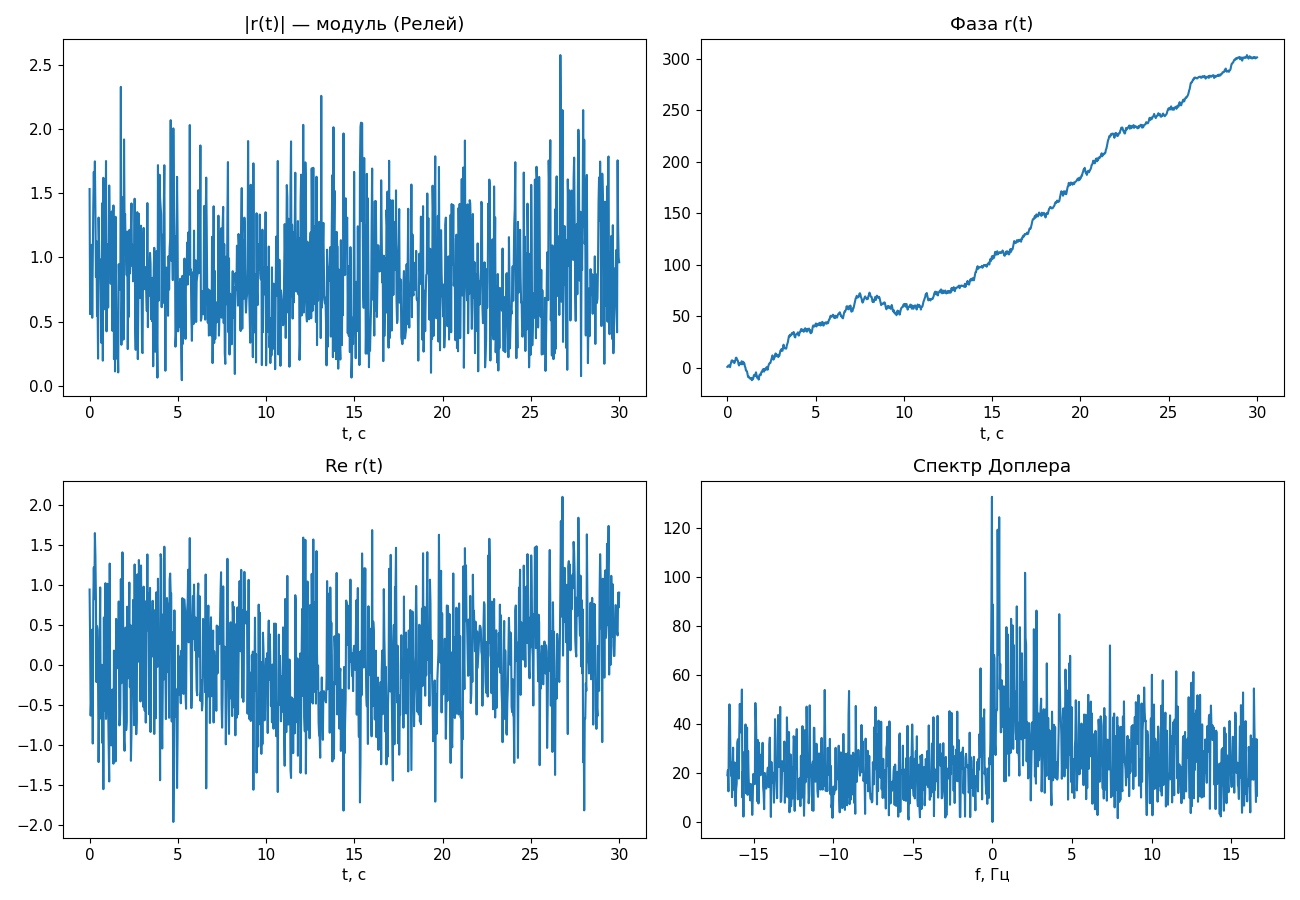
\includegraphics[width=\textwidth]{radio_part2.png}
    \caption{Часть 2: модуль, фаза, вещественная часть и спектр Доплера
             при многолучевом распространении}
    \label{fig:part2}
\end{figure}

\textbf{Модуль.} В отличие от части~1, $|r(n)|$ хаотически флуктуирует,
наблюдаются глубокие провалы (замирания) — характерный признак релеевского
канала.

\textbf{Фаза.} Фаза также случайно изменяется, поскольку сумма множества
лучей с разными набегами фаз даёт случайную комплексную величину.

\textbf{Спектр Доплера.} Вместо одиночной линии наблюдается размытая
полоса в интервале $[-f_D, +f_D]$, где $f_D = V/\lambda$ — максимальный
доплеровский сдвиг. Разные лучи приходят под разными углами $\theta_i$,
поэтому их доплеровские частоты $f_{Di} = (V/\lambda)\cos\theta_i$
распределены по полосе. Форма спектра близка к классическому
«доплеровскому спектру Кларка» (U-образная).

\subsection{Статистические характеристики модуля}

\textbf{Гистограмма.} На рисунке~\ref{fig:hist} приведена нормированная
гистограмма модуля $|r|$ (плотность вероятности, нормировка на количество
точек трека) и теоретическая кривая распределения Рэлея:
\begin{equation}
    p_{|r|}(x) = \frac{x}{\sigma^2}\exp\!\left(-\frac{x^2}{2\sigma^2}\right),
    \quad x \ge 0,
\end{equation}
где $\sigma^2 = \mathbb{E}|r|^2/2$.

\begin{figure}[h]
    \centering
    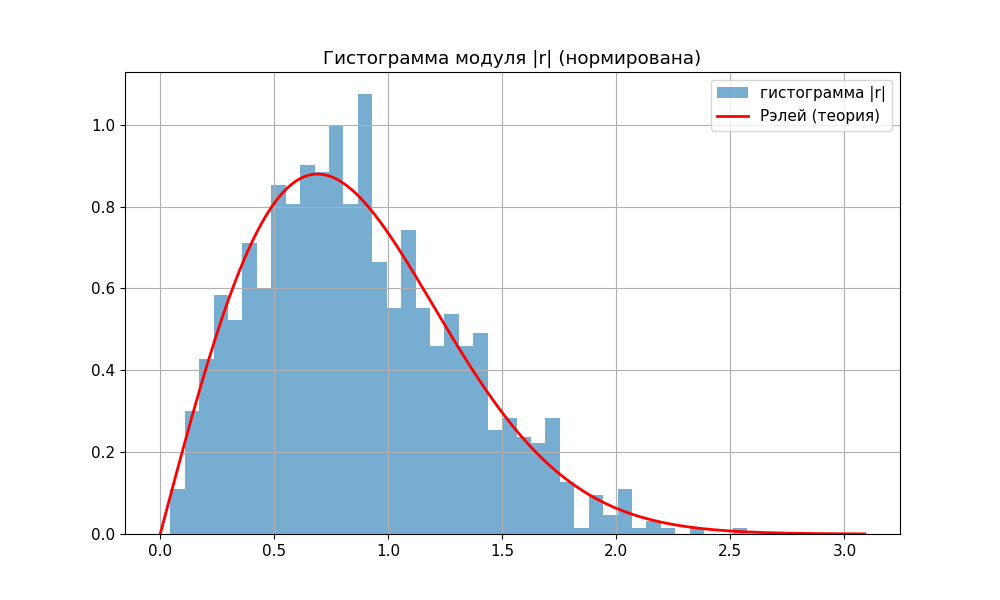
\includegraphics[width=0.8\textwidth]{radio_hist.png}
    \caption{Гистограмма модуля $|r|$ и теоретическое распределение Рэлея}
    \label{fig:hist}
\end{figure}

\textbf{Функция распределения.} На рисунке~\ref{fig:cdf} приведены
эмпирическая CDF модуля и теоретическая CDF Рэлея:
\begin{equation}
    F_{|r|}(x) = 1 - \exp\!\left(-\frac{x^2}{2\sigma^2}\right).
\end{equation}

\begin{figure}[h]
    \centering
    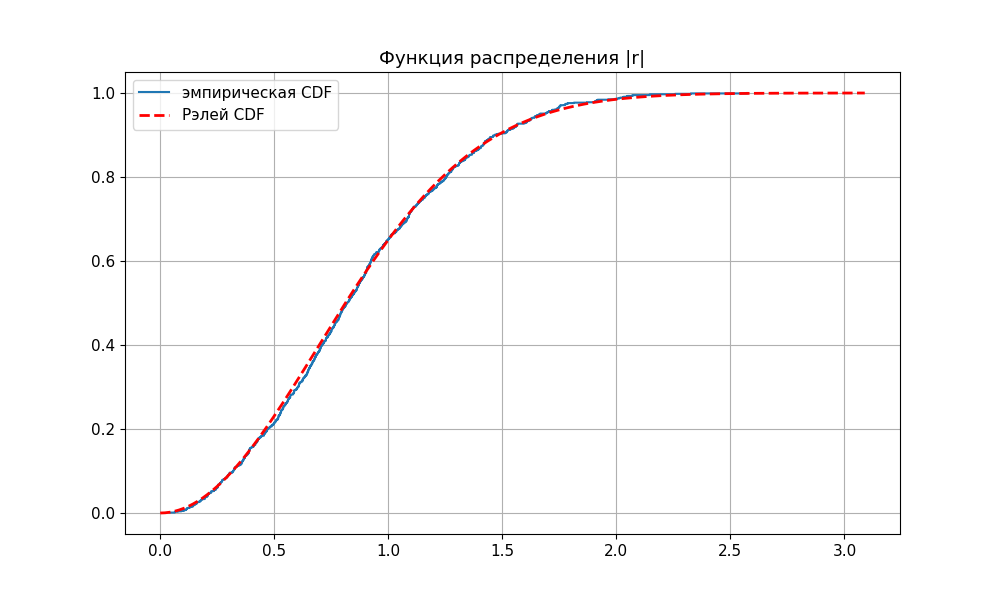
\includegraphics[width=0.8\textwidth]{radio_cdf.png}
    \caption{Эмпирическая и теоретическая функции распределения модуля $|r|$}
    \label{fig:cdf}
\end{figure}

Совпадение эмпирических кривых с теоретическими подтверждает, что при
большом числе независимых лучей распределение модуля принимаемого сигнала
стремится к рэлеевскому (следствие центральной предельной теоремы).

\textbf{Числовые оценки.} Средняя мощность $\mathbb{E}|r|^2 \approx 1$,
среднее значение $|r|$ близко к $\sigma\sqrt{\pi/2}$, дисперсия — к
$(2-\pi/2)\sigma^2$. Эти оценки совпадают с теоретическими для закона
Рэлея.

\subsection{Автокорреляционная функция}

Автокорреляционная функция принятого сигнала по треку:
\begin{equation}
    R_r(\tau) = \mathbb{E}\bigl[r(t)\,r^*(t+\tau)\bigr]
\end{equation}
(в дискретной форме — нормированная корреляция последовательности $r(n)$
с её сдвинутой копией). График приведён на рисунке~\ref{fig:acf}.

\begin{figure}[h]
    \centering
    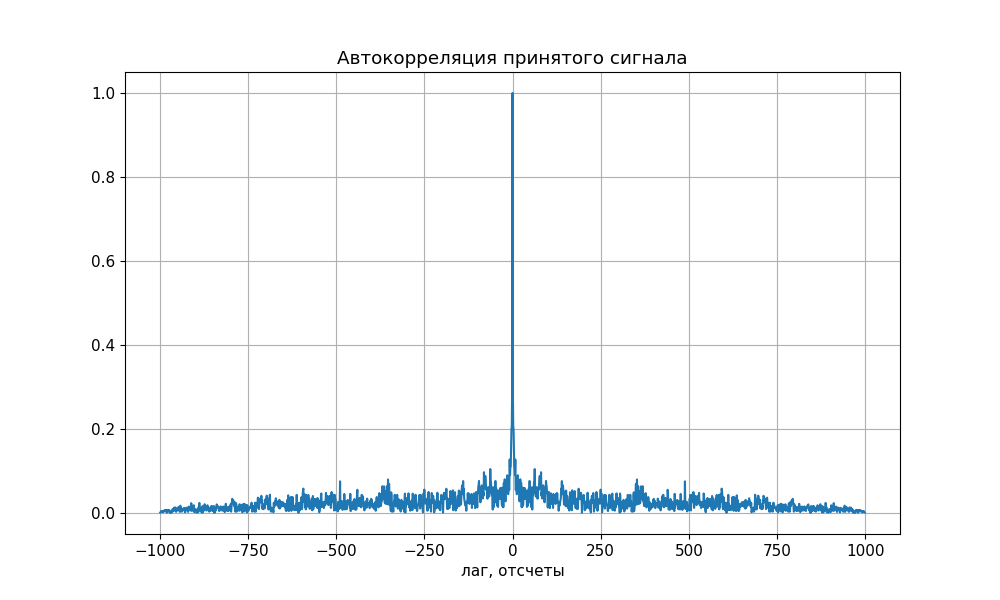
\includegraphics[width=0.8\textwidth]{radio_acf.png}
    \caption{Автокорреляционная функция принятого сигнала}
    \label{fig:acf}
\end{figure}

Для релеевского канала с доплеровским спектром Кларка теоретическая
автокорреляция имеет вид $R_r(\tau) = J_0(2\pi f_D\tau)$, где $J_0$ —
функция Бесселя нулевого порядка. Время когерентности канала
$T_c \approx 1/f_D$. Эмпирическая АКФ спадает за время порядка
$T_c$, что согласуется с теорией.

\section{Контрольные вопросы}

\subsection{Почему при одном луче амплитуда постоянна, а при многих —
флуктуирует?}

При одном луче принимаемый сигнал $r = e^{-jkd}$ имеет единичный модуль
при любом $d$: меняется только фаза. При многих лучах сумма
$r = \sum_i e^{j\varphi_i}$ — это сумма случайных комплексных векторов
с равномерно распределёнными фазами. По центральной предельной теореме
её действительная и мнимая части асимптотически гауссовы с нулевым
средним, а модуль распределён по Рэлею — отсюда флуктуации и глубокие
провалы.

\subsection{От чего зависит доплеровский сдвиг и почему в части 1
спектр — одна линия, а в части 2 — полоса?}

Доплеровский сдвиг $f_D = (V/\lambda)\cos\theta$ зависит от скорости
$V$, длины волны $\lambda$ и угла $\theta$ между направлением движения
и направлением на источник. В части~1 источник один (BS), угол
фиксирован, поэтому сдвиг один и спектр — одиночная линия. В части~2
лучи приходят с разных направлений (через разные рассеиватели), углы
$\theta_i$ разные, поэтому набор доплеровских частот заполняет полосу
$[-V/\lambda, +V/\lambda]$.

\subsection{Почему шаг дискретизации по расстоянию выбирается как
$\Delta x = \lambda/F$?}

Шаг $\Delta x$ задаёт дискретизацию по времени $t_s = \Delta x/V$ и,
следовательно, частоту дискретизации $f_s = V/\Delta x$. Чтобы
доплеровский сдвиг $f_D = V/\lambda$ не превышал частоту Найквиста
$f_s/2$, необходимо $V/\lambda < V/(2\Delta x)$, то есть
$\Delta x < \lambda/2$. Выбор $\Delta x = \lambda/16$ даёт большой запас
($F = 16 \gg 2$) и обеспечивает корректное восстановление фазы без
алиасинга.

\subsection{Как по гистограмме модуля убедиться, что канал релеевский?}

Нужно нормировать гистограмму на количество точек (получить плотность
вероятности), оценить $\sigma^2 = \mathbb{E}|r|^2/2$ по выборке и
наложить теоретическую кривую Рэлея $p(x) = (x/\sigma^2)e^{-x^2/(2\sigma^2)}$.
Совпадение гистограммы с кривой (а также совпадение эмпирической CDF
с $F(x) = 1 - e^{-x^2/(2\sigma^2)}$) и есть проверка релеевского закона.
Дополнительно можно использовать критерий согласия Колмогорова—Смирнова.

\subsection{В чём смысл автокорреляционной функции принимаемого сигнала?}

АКФ показывает, насколько быстро сигнал «забывает» себя при сдвиге по
времени, то есть определяет время когерентности канала $T_c$. Для
релеевского канала $R_r(\tau) = J_0(2\pi f_D\tau)$, и $T_c \sim 1/f_D$.
Чем выше скорость абонента или несущая частота, тем больше $f_D$ и тем
быстрее замирания, тем меньше $T_c$ — это важно для выбора длины
пилот-последовательности, интервала канального оценивания и т.п.

\section*{Вывод}
\addcontentsline{toc}{section}{Вывод}

В ходе работы освоено имитационное моделирование радиоканала подвижной
связи. Для прямого луча показано, что принимаемый сигнал имеет постоянную
амплитуду и линейно меняющуюся фазу, а его доплеровский спектр
представляет собой одиночную линию на частоте $f_D = V/\lambda \approx
66{,}7$~Гц. Для многолучевого сценария с 200 рассеивателями показано, что
модуль принимаемого сигнала флуктуирует и подчиняется распределению
Рэлея, доплеровский спектр размывается в полосу $[-V/\lambda, V/\lambda]$,
а автокорреляционная функция спадает за время когерентности порядка
$1/f_D$. Полученные результаты согласуются с теорией релеевских замираний
и подтверждают корректность модели.

\endinput